\section{Machine Learning}
\label{sec:ml}

\textbf{Goal}: as in Figure~\ref{fig:ideal} we want a machine learning algorithm $\mathcal{L}$ that predict the \textit{action label} $a_i$ given the \textit{action's flows} $A_i = [F_1,\dots, F_n]_i$.

\begin{figure}[h]
 \centering
 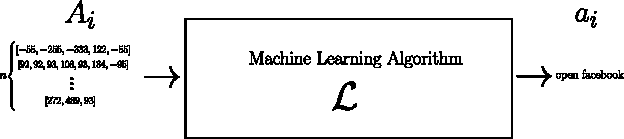
\includegraphics{images/ideal}
 \caption{\small{The ideal model predicti the label $a_i$ for the a new input instance $A_i$.}}
 \label{fig:ideal}
\end{figure}

Given the fact that each action generates multiple flows of different lengths, we know that standard supervised learning approaches are hard to apply. To see why standard approaches would not work we need to think about the structure of the input and output spaces. Our output space i.e. what we want to predict would be the \textit{action label} $a_i$, while our input space, i.e. the predictors, would be the flows generated by $a_i$ which we denote as $[F_1,\dots,F_n]_i $. One way we could represent flows as features would be to have a feature for each flow $F_j$ generated by the action $a_i$, and the value of the $j$-th feature would be the sequence of byte sizes of the flow $[p_1,\dots, p_m]_j$. Because of the different number of flows for each action  $n$ we would immediately see that each row could possibly have a different number of features. The main problem of this approach, other than the just mentioned diverse dimensionality, is that we are artificially defining features with no real justification; in other words, we have no reason to associate the first flow of an action $A_i$ with the first flow of another action $A_j$ by viewing them as the first feature of their respective samples.


To overcome this obstacle the original authors applied a two stage process. In the first stage, by using an unsupervised clustering algorithm, they addressed their missing knowledge about the number of flows and their features. The objective is to identify some kind of intermediate representation of the data $\Phi(A_i)$ that can be exploited by the second stage of the process, which will perform a canonic classification (Figure~\ref{fig:actual}). 
In the remainder of this section we describe the algorithms used in the two stage process and my personal implementation.\todo{decidere come strutturare sta roba.}

\begin{figure}[h]
 \centering
 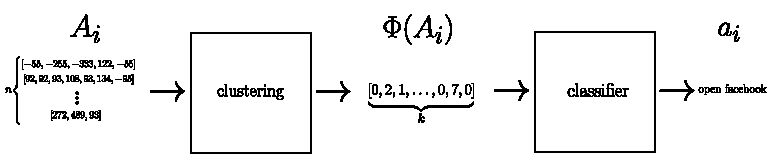
\includegraphics{images/actual}
 \caption{\small{The two step classification of a new sample; first the new sample $A_i$ goes through the clustering algorithm which computes the intermediate representation $\Phi(A_i)$, then $\Phi(A_i)$ is used by the classifier to predict the correct label $a_i$. $k$ is the number of clusters, a more detailed description of $k$ and $\Phi$ can be found in \ref{subsubsec:hac}, \ref{subsubsec:fexc}.}}
 \label{fig:actual}
\end{figure}

\subsection{Clustering}
In the typical unsupervised clustering scenario the goal of the algorithm is to find $k$ groups called clusters, where the \textit{inter-cluster} similarity is very low while the \textit{intra-cluster} similarity is maximized, meaning that samples belonging to one clusters are very similar to each other while still being very different from samples belonging to other clusters. Notice that the number of clusters $k$ and the similarity function between samples have to be explicitly defined by the teacher. The input of the clustering algorithm is usually the whole datset while its output is a list of intergers $[c_i,\dots, c_N]$ where $N$ is the total number of samples and $c_i \in [1;k]$ is a an integer number that denotes the cluster to which the $i$-th sample has been assigned by the algorithm.

\subsubsection{Hierarchical Agglomerative Clustering}
\label{subsubsec:hac}
In this specific instance I used (as suggeseted in the papers) a \textbf{Hierachical Agglomerative Clustering}, \textbf{HAC} for short. HAC starts by creating a cluster for each flow; at each step HAC reduces the number of clusters by merging (agglomerative) the closest clusters together based on the distance function and other parameters; HAC will stop whenever the desired number of clusters $k$ is reached. The structure that HAC exploits can be seen as a tree (hierachical), that structure is called dendrogram; in Figure \ref{fig:dendro} we can see the dendrogram for 20 samples (i.e. 20 flows). In my implementation the input consists in all the flows contained in the dataset\footnote{We are just using flows now, the concept of ``actions'' is being ignored for the moment since it is not really needed for the clustering stage.}, the number of clusters $k$ is set to $50$, and the distance function used to compute similarity between flows is the Dynamic Time Warping described in the following paragraph.

\begin{figure}[!h]
 \centering
 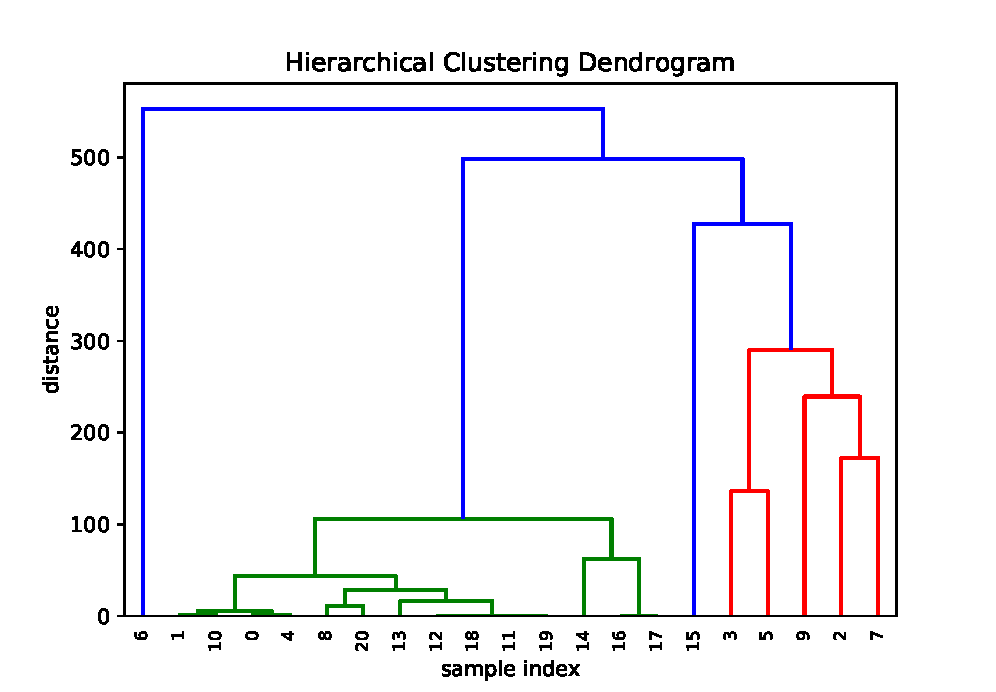
\includegraphics[scale=0.5]{images/dendrogram}
 \caption{\small{Dendrogram for 20 flows; the number of clusters can be seen by counting how many vertical lines get crossed by an imaginary horizontal line. Different horizontal lines will of course determine different clusters and different distance measures; the dendrogram allows the designer to decide at what level to draw the line i.e. which value to assign to $k$ by looking at the distance value and at the hierarchy itself.}}
 \label{fig:dendro}
\end{figure}

\subsubsection{Dynamic Time Warping}
\label{subsubsec:dtw}
\textbf{Dynamic Time Warping} or \textbf{DTW} is an algorithm generally used to find the best match between two time series even when they have different lengths and/or have repetitions or deletions in them. If we view every single flow $F_i$ as a series of packets $[p_1,\dots p_m]_i$, we can use DTW to measure how similar two flows are. This similarity measure is needed by the HAC algorithm to compute the distances between clusters.

\subsubsection{Feature Extraction}
\label{subsubsec:fexc}
The HAC output is, as stated before, a list of $N$ integers $[c_1,\dots, c_N]$ where $c_i$ is the cluster assigned to the $i$-th input sample. This is different from what is reported in Figure \ref{fig:ideal}, in fact the clustering result needs to be rearranged before being given as input to the classifier. The aim of the rearrangement is to actually generate a new intermediate dataset where the target we want to predict are still the actions' labels but the features are now different. We generate $k$ features for each action $A_i$; the value of the $j$-th feature is the number of flows of $A_i$ that ended in the $j$-th cluster during the clustering algorithm. This whole process composed by the \textit{clustering} and the final rearrangement is what we call feature extraction and denote with the symbol $\Phi$, so $\Phi(A_i)$ is the intermediate representation of $A_i$ and is considered to be a single input sample of the new intermediate dataset.

\begin{table}[]
\label{tab:newdataset}
\centering
\begin{tabular}{@{}lcccc@{}}
\toprule
\textbf{action\_label}     & \multicolumn{1}{l}{\textbf{C1}} & \multicolumn{1}{l}{\textbf{C2}} & \multicolumn{1}{l}{\textbf{\dots}} & \multicolumn{1}{l}{\textbf{C50}} \\ \midrule
open facebook              & 0                               & 11                              & \dots                              & 6                                \\
writing search             & 1                               & 1                               & \dots                              & 5                                \\
back to news               & 0                               & 0                               & \dots                              & 0                                \\
open facebook              & 0                               & 9                               & \dots                              & 5                                \\
\multicolumn{1}{c}{\vdots} & \vdots                          &                                 & \vdots                             & \vdots                           \\ \bottomrule
\end{tabular}
\caption{\small{Format of the new dataset. We can see that 11 flows of the first action ended up in cluster number 2, while 6 of them ended up in the last cluster.}}
\end{table}

\subsection{Classification}
Now that we have a suitable dataset we can apply a supervised classification machine learning algorithm. In this scenario we split the data in two disjunct sets: \textit{training} and \textit{test set}; the first will be used to train the classifier while the other will test if the algorithm actually learned the concept that correlates the intermediate representation $\Phi(A_i)$ to the label $a_i$. The machine learning algorithm chosen is \textbf{Random Forest}.

\subsubsection{Random Forest Classifier}
The Random Forest Classifier is, as the name says, a classifier; its two main features can also be explained by analyzing its name:
\begin{itemize}
 \item \textbf{Forest}: it is a collection of decision trees (which are (\textit{weak}) classifiers themselves); if we want to classify a new instance on an already trained forest, what happens under the hood is that the forest will pass that instance to all of its trees and each one of them will return a prediction for that instance; the output of the forest will be the prediction voted the most by its trees.\footnote{Some variants will weight the vote of each tree differently based on their performance.}
 \item \textbf{Random}: in Random Forest there are two degrees of randomness; during training phase each tree has to be build using:
 \begin{itemize}
  \item a random subset of the total input data;
  \item a random subset of features extracted from all the features available (usually $\sqrt{\text{total number of features}}$).
 \end{itemize}
\end{itemize}

To better understand how Random Forest works it is worth mentioning the basic structuture and mechanisms we find in Decision Trees. 

\paragraph{Structure of Decision Trees}
\begin{itemize}
 \item \textbf{nodes}: each internal node (root node included) can be represented by the subset of the samples it is working with (the root node is working with the whole dataset) and by the decision that has to be made at that node; the decision is just a boolean expression that gets applied to the all elements of the current subset. 
 \item \textbf{arcs}: the arcs are the possible outcomes of the decision at a given node; the elements of the subset of the node will be sent down the arc (and the following sub-tree) they ``satisfy''.
 \item \textbf{leaf nodes}: leaf nodes are predictions (this means they are possible values of $a$ or \textit{action labels}), a leaf node is formed when all the elements of a given node have the same class/target/$a$/\textit{action label}.
\end{itemize}

\paragraph{Mechanisms of Decision Trees}
The aim of the Decision Tree is to generate at each node the purest possible subsets, to do so it uses (im)purity measures (Information Gain) or dispersion measures (Gini Index). At each node only one feature is tested, the outgoing arcs of a node are the number of possible values that the feature can assume (if discrete) or a threshold value (if real), in which case only two arcs will be generated. Both the feature and the threshold (if any) are chosen based on the criteria cited previously. Adding to what have been said in the previous paragraph: a leaf node can be formed also when there are no more features to test (they have all been tested in previous nodes), in this case the prediction of the leaf node will be the \textit{action label} with higher frequency on that subset. A part of a Decision Tree can be seen in Figure \ref{fig:tree}, the colors and their intenisity are used to highlight which \textit{action label} is more frequent at each node.

\begin{figure}[!h]
 \centering
 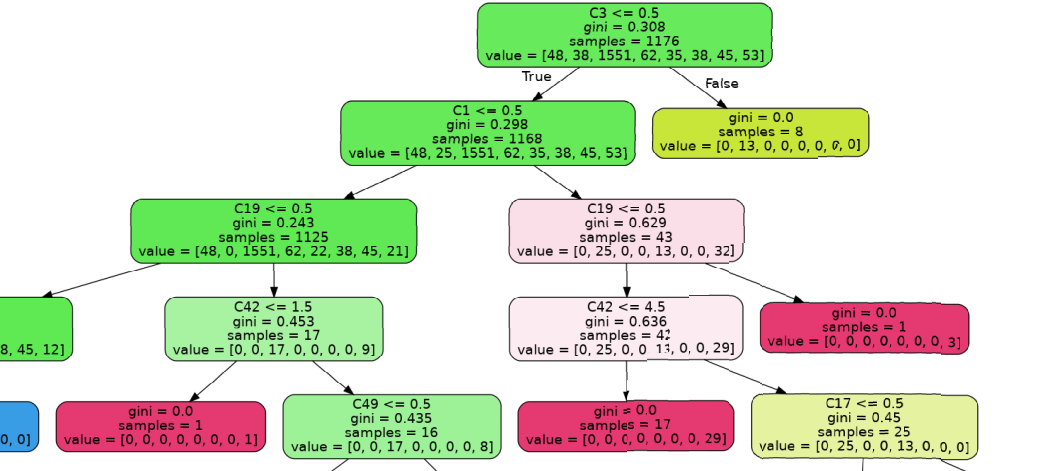
\includegraphics[scale=0.4]{images/tree}
 \caption{\small{Small part of a single tree of the forest. At each node the value of a given feature is tested, the arcs opening to the left satisfy the condition while those to the right do not.}}
 \label{fig:tree}
\end{figure}


